For this study, four coastal towns of Denmark were selected to investigate the impact of the storm surge in October 2023. The four areas were Aabenraa, Gedser Havn, Hesnæs and Præstø.\\

A total of eight municipalities were contacted prior to selection. These include Aabenraa, Faaborg-Midtfyn, Guldborgsund, Haderslev, Stevns, Sønderborg and Vordingborg. The selection of potential sites was based on a table from the Danish Meteorological Institute (DMI)  \citep{damberg_vaerste_2023} of the highest recorded sea water levels in Denmark during the 2023 storm surge.
Out of the eight municipalities, three (Aabenraa, Guldborgsund and Vordingborg) were selected for further cooperation based on available data. Guldborgsund provided data from four locations in the municipality, but only two sites (the coastal towns of Gedser Havn and Hesnæs) were chosen based on their higher measured water level during the storm surge and the scope of the initial study.\\

The four selected study areas are located along the south coast of Denmark. Figure \ref{Figur: Oversigtskort} visualises the locations of the areas in the country.
\begin{figure}[H]
	\centering
	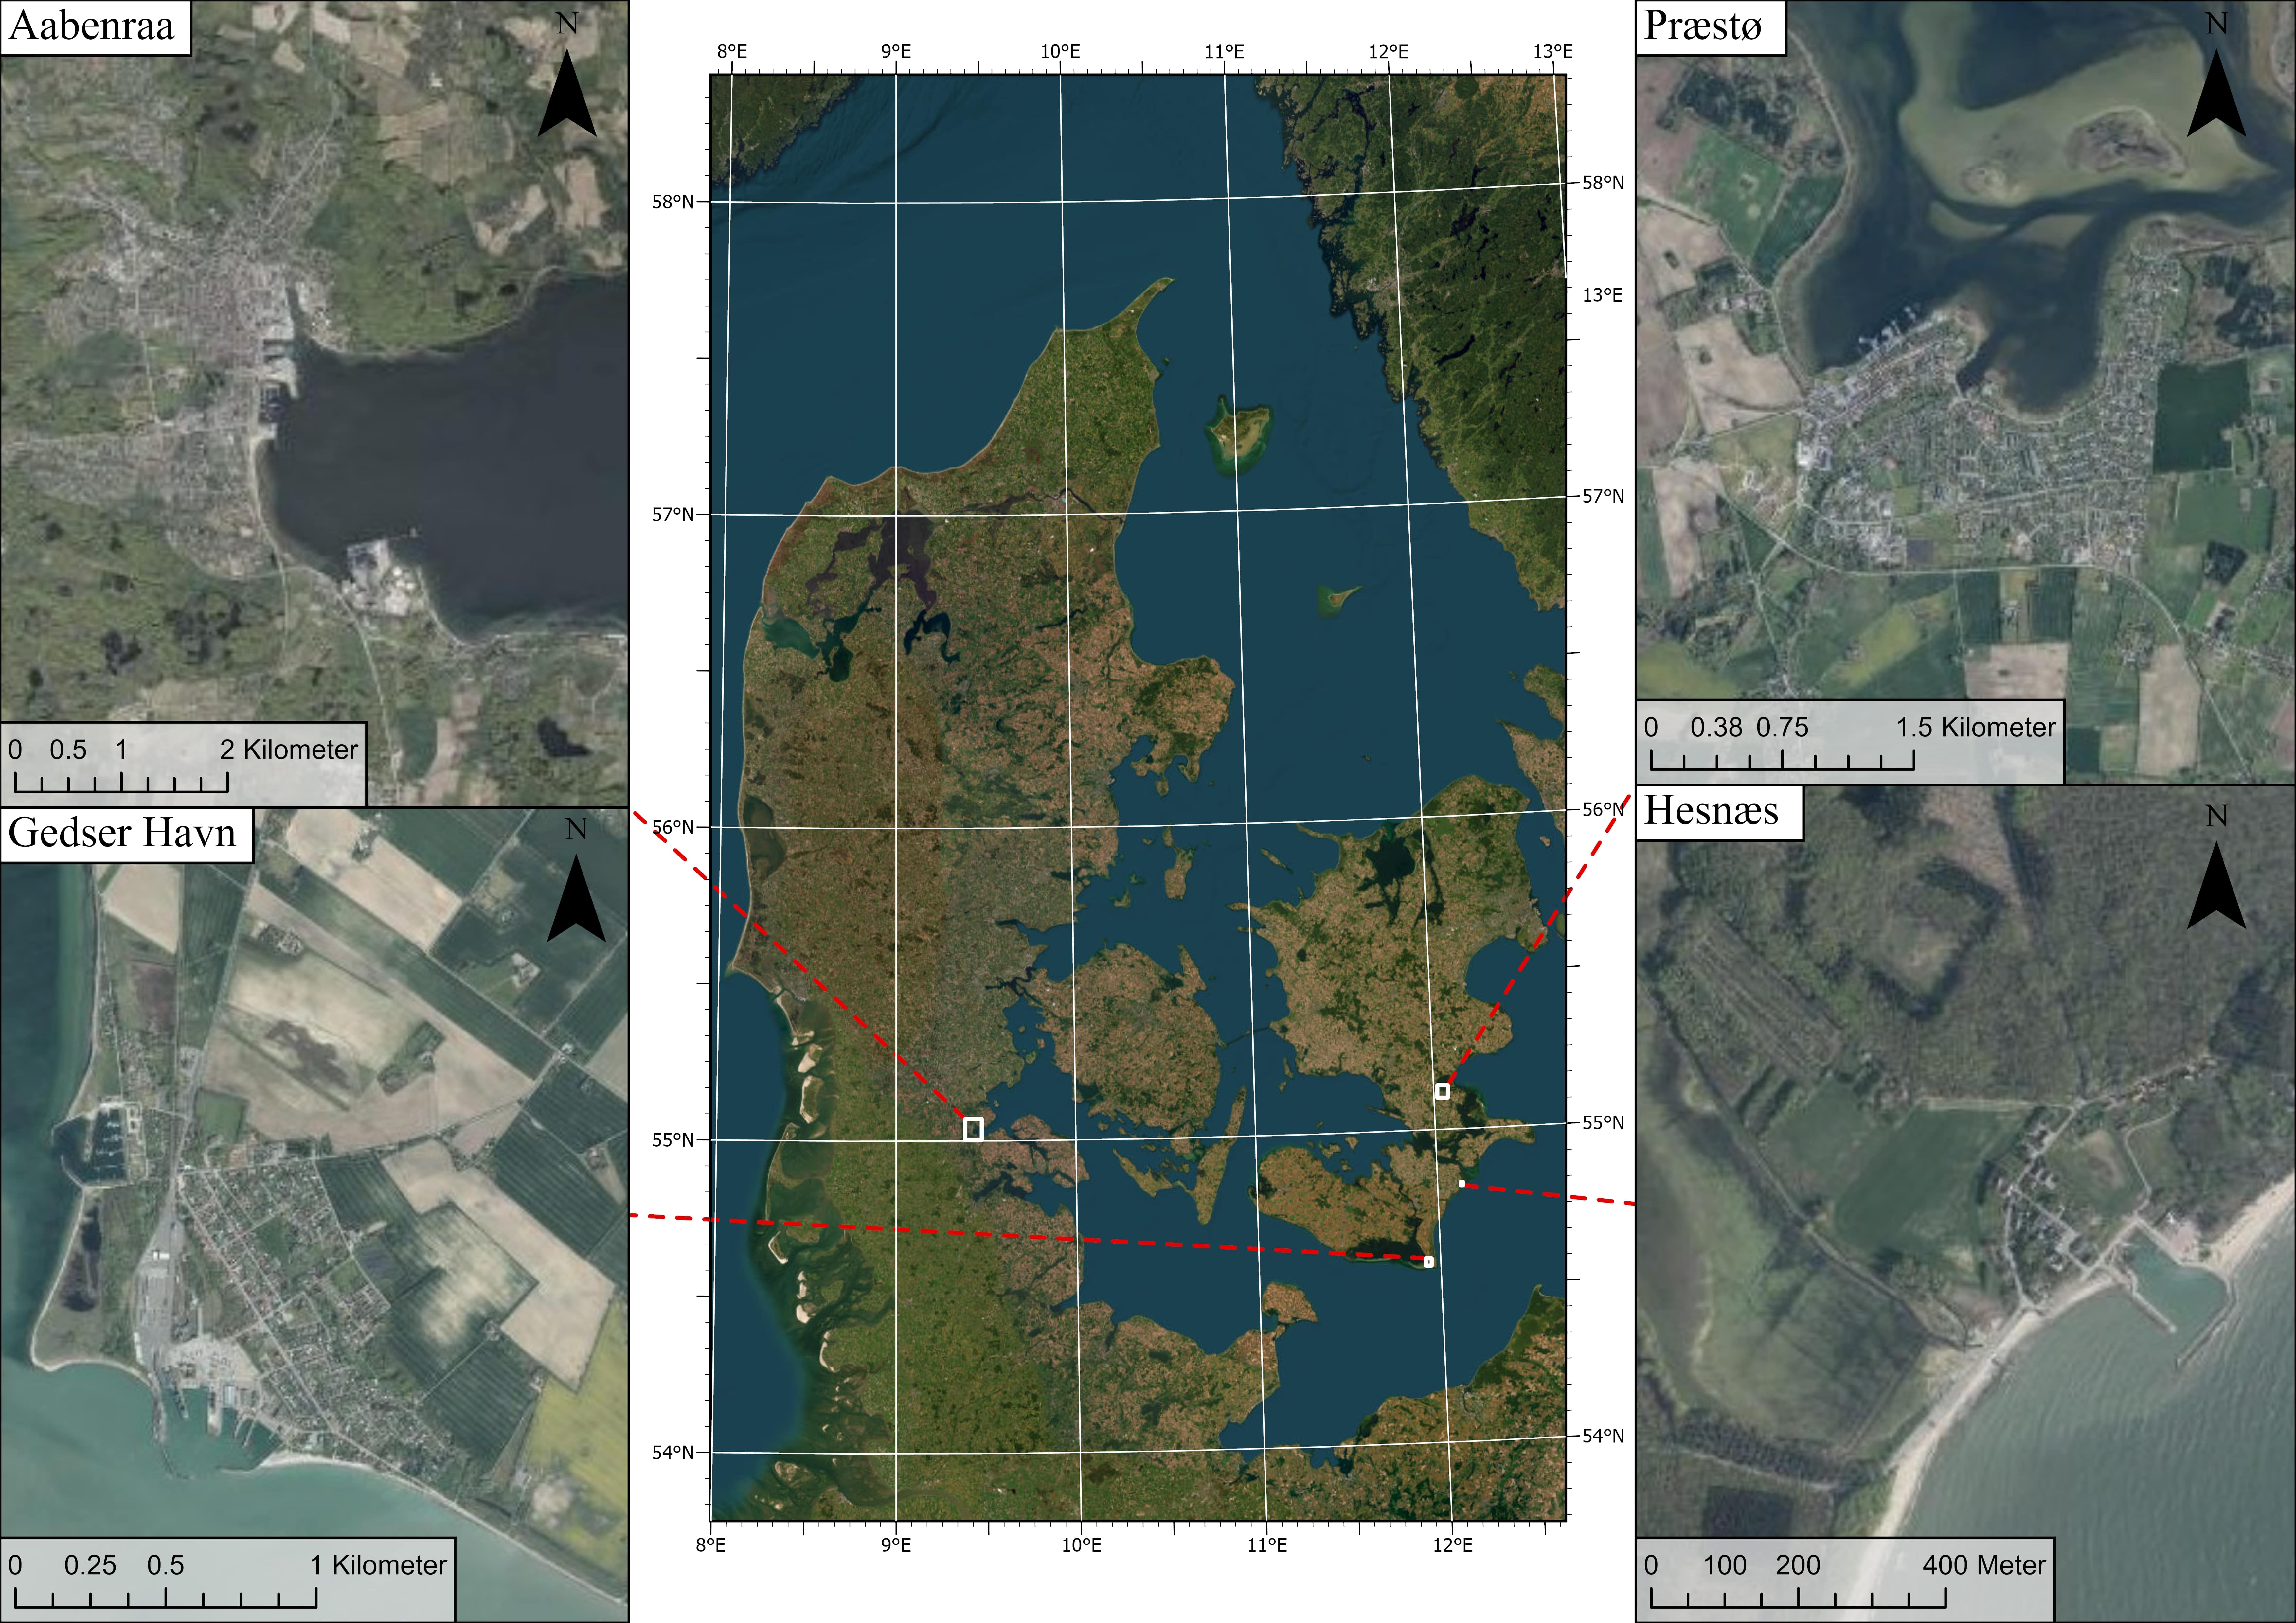
\includegraphics[width=1\linewidth]{images/studieområder/oversigtskort.jpg}
	\caption{Oversigtskort over studieområderne: Aabenraa, Gedser Havn, Hesnæs og Præstø. Baggrundskort fra ESRI og Klimadatastyrelsen.}
	\label{Figur: Oversigtskort}
\end{figure}

\noindent
\textit{Aabenraa}\\
Aabenraa is a city in southeastern Jutland. The city is located in the Aabenraa municipality at the end of the approximately 10 km long Aabenraa Fjord. The city as a population of 16,500 and is the ninth largest city in the Region of Southern Denmark \citep{danmarks_statistisk_mobile_nodate}. The city consists of two industrial ports, Aabenraa and Ensted, and both are important for shipping traffic with 380 ships calling at port in 2022 \citep{aabenraa_havn_aabenraa-havn-talogfakta2022_2022}.\\
Aabenraa recorded the highest official water level during the storm surge of 2.16 metres above DVR90 (figure \ref{Subfig: Aabenraa vandstand}).\\

\noindent
\textit{Gedser Havn}\\
Gedser Havn is a small town on the southern tip of the island of Falster in Guldborgsund municipality. Gedser Havn serves as an active fishing port and as a ferry port to the German port of Warnemünde near the city of Rostock. The town had a population of 670 in 2024 \citep{danmarks_statistisk_mobile_nodate} and is Denmark's southernmost town.\\
During the storm surge, a water level rise of 1.89 metres above DVR90 was recorded in Gedser Havn (figure \ref{Subfig: Gedser vandstand}), the highest recorded water level since 1892, and that suspended ferry traffic to Germany until the morning of the 21st of October \citep{tiirikainen_sadan_2023}.
\begin{figure}[H]
	\begin{subfigure}[b]{0.5\textwidth}
		\centering
		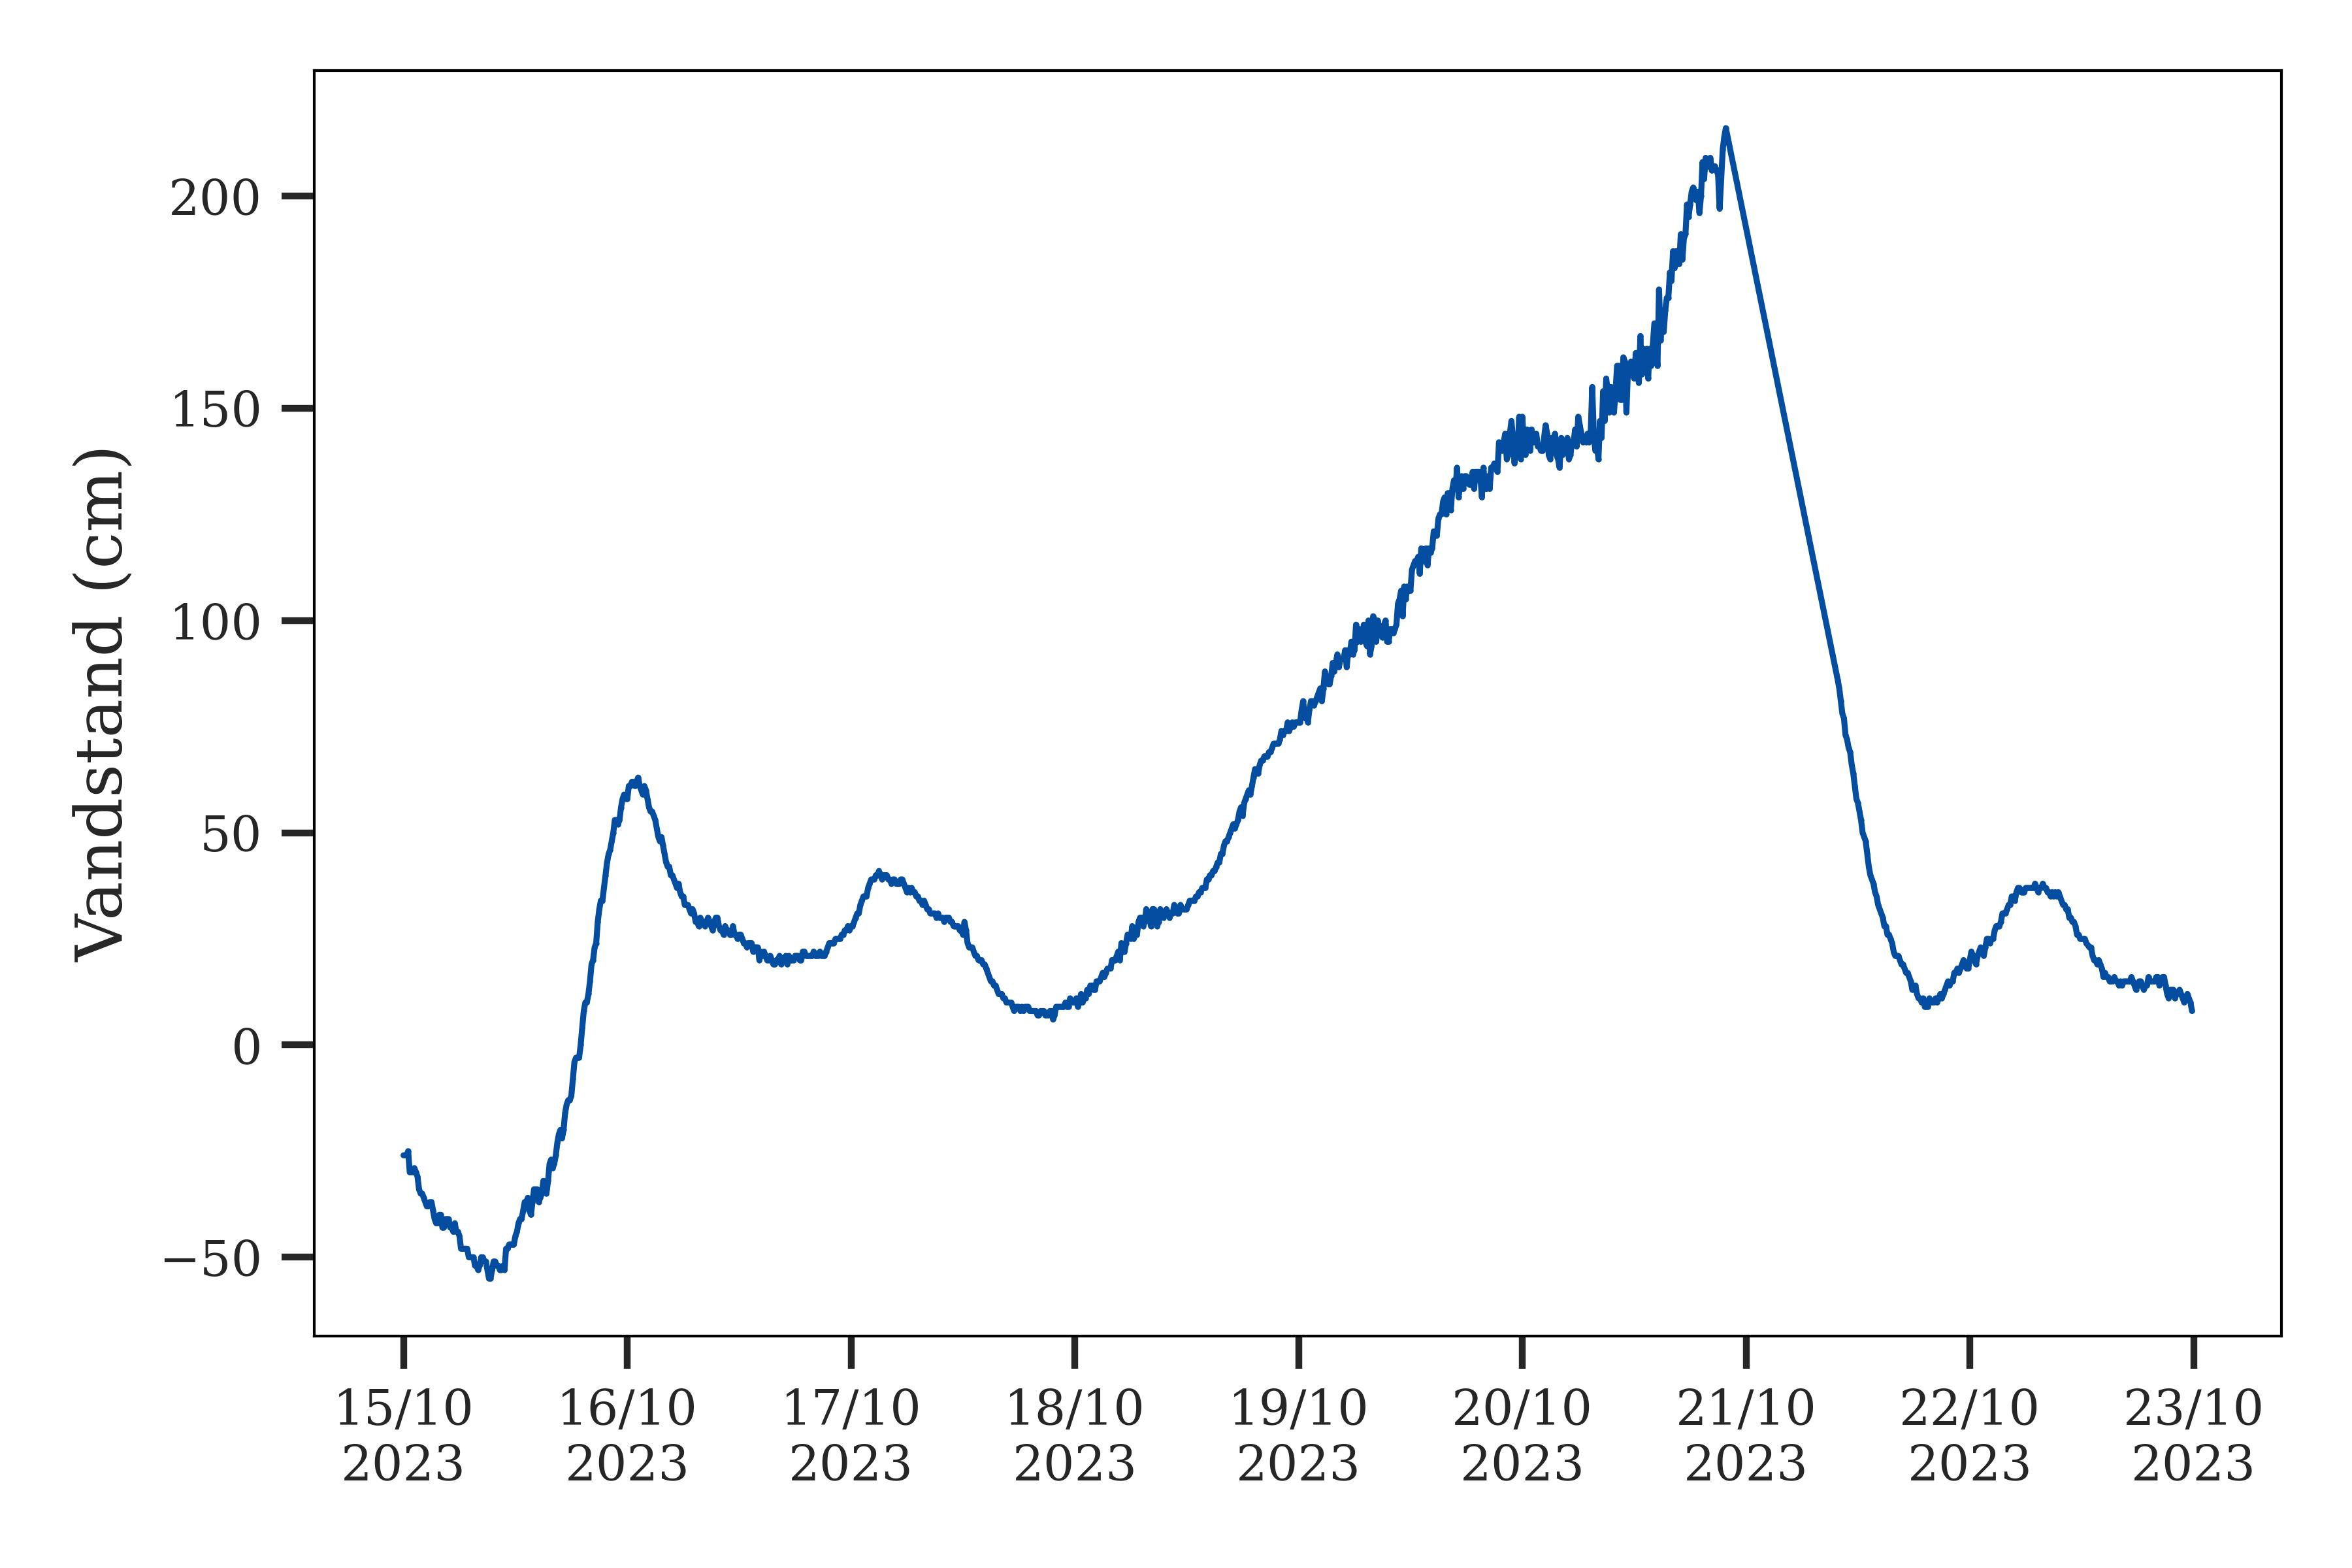
\includegraphics[width=1\textwidth]{images/studieområder/vandstands_grafer/vandstand_aabenraa_vandstandsplot.jpg}
		\caption{}
		\label{Subfig: Aabenraa vandstand}
	\end{subfigure}
	\hspace{0.2cm}
	\begin{subfigure}[b]{0.5\textwidth}
		\centering
		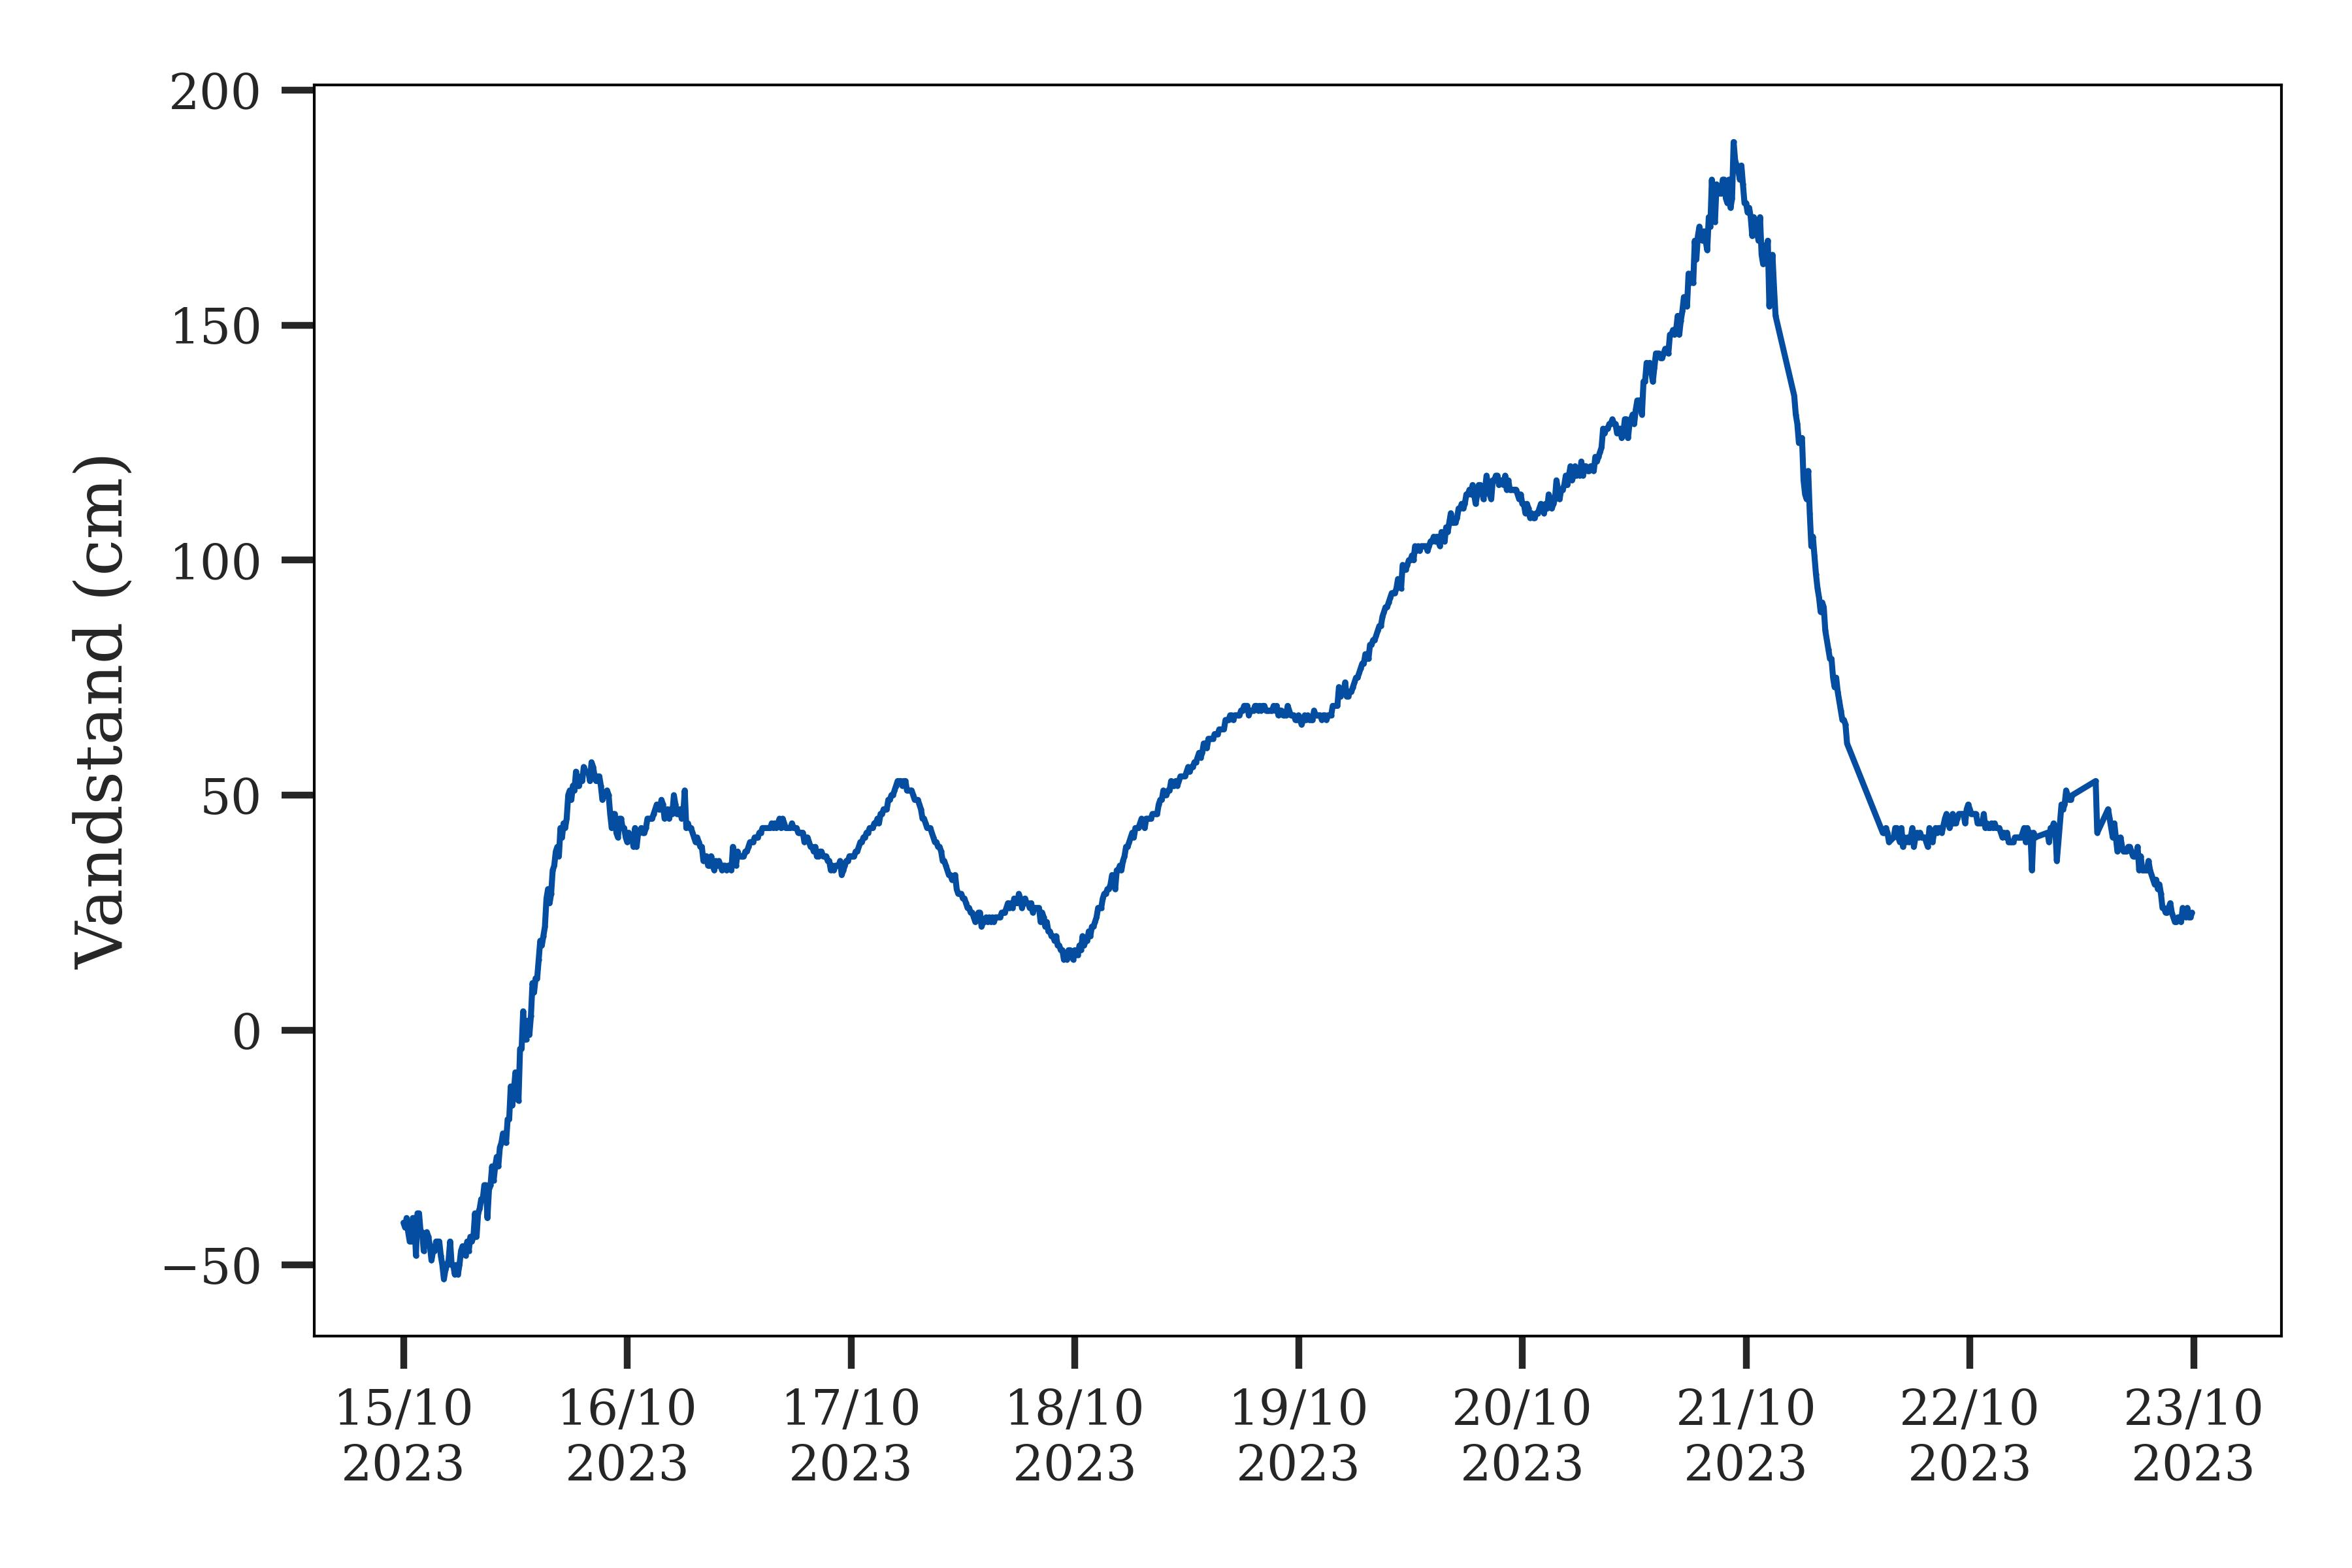
\includegraphics[width=1\textwidth]{images/studieområder/vandstands_grafer/vandstand_gedser_vandstandsplot.jpg}
		\caption{}
		\label{Subfig: Gedser vandstand}
	\end{subfigure}
	\vspace{0.2cm}
	\begin{subfigure}[b]{0.5\textwidth}
		\centering
		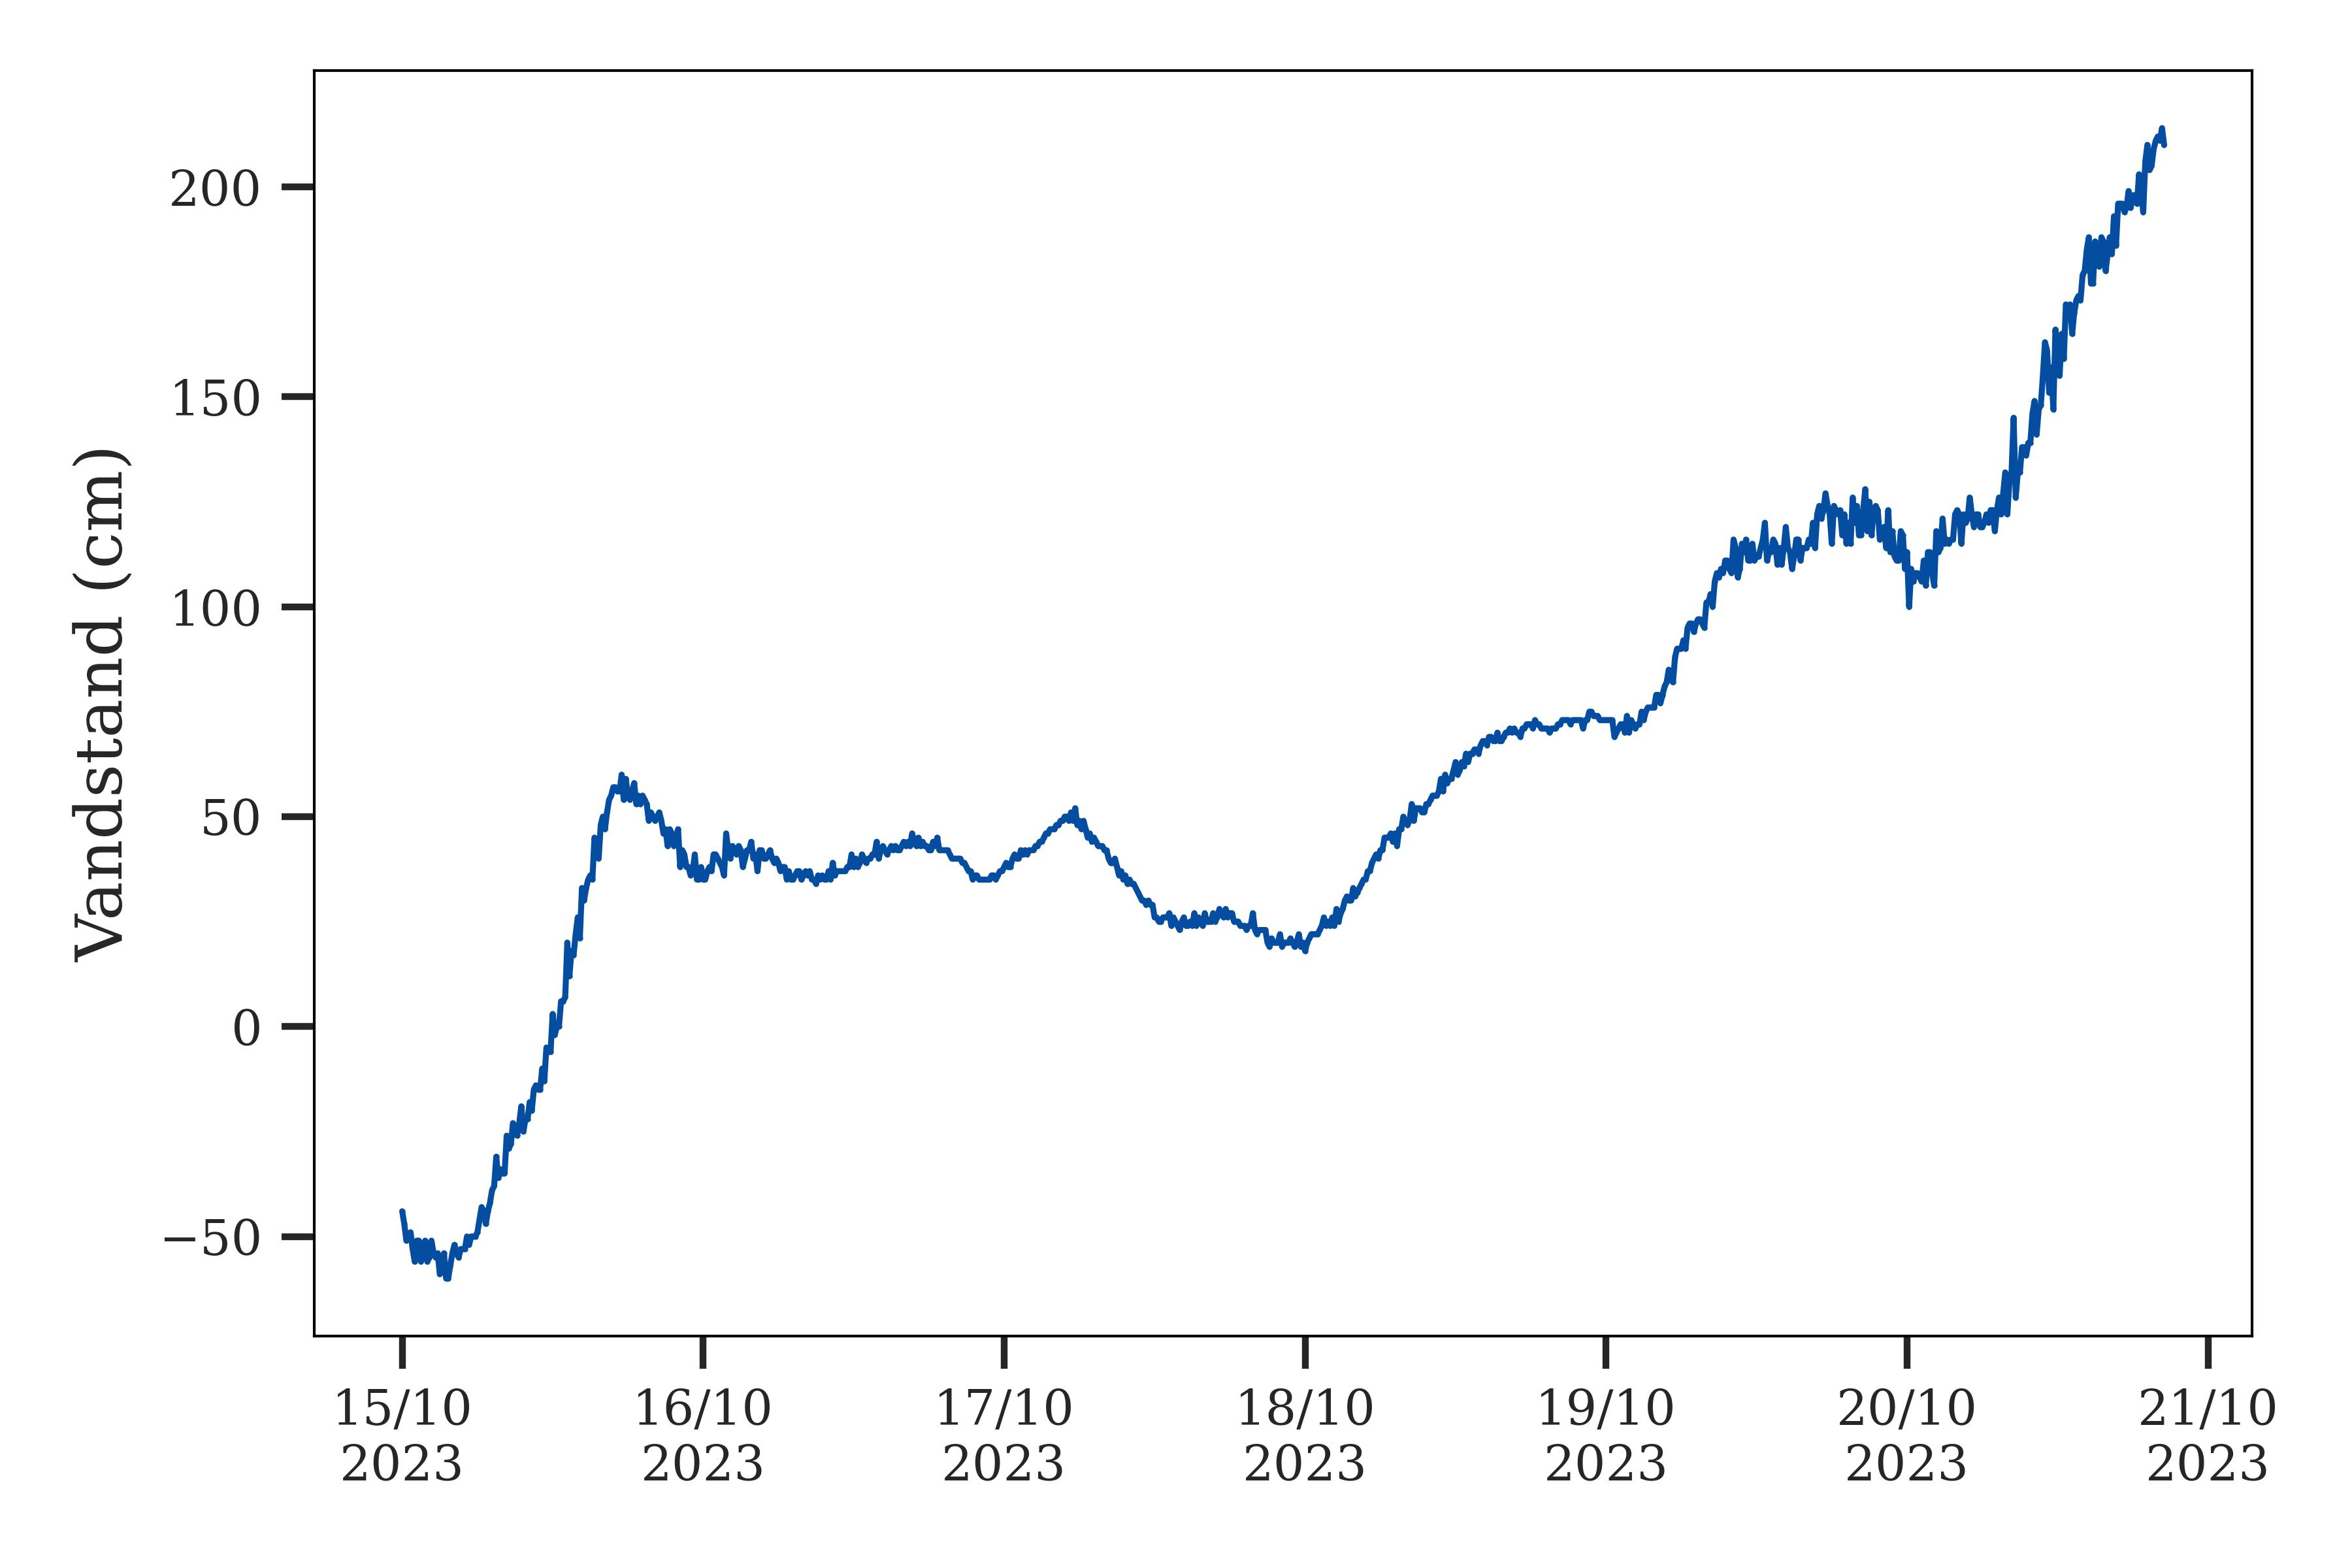
\includegraphics[width=1\textwidth]{images/studieområder/vandstands_grafer/vandstand_hesnaes_vandstandsplot.jpg}
		\caption{}
		\label{Subfig: Hesnæs vandstand}
	\end{subfigure}
	\hspace{0.2cm}
	\begin{subfigure}[b]{0.5\textwidth}
		\centering
		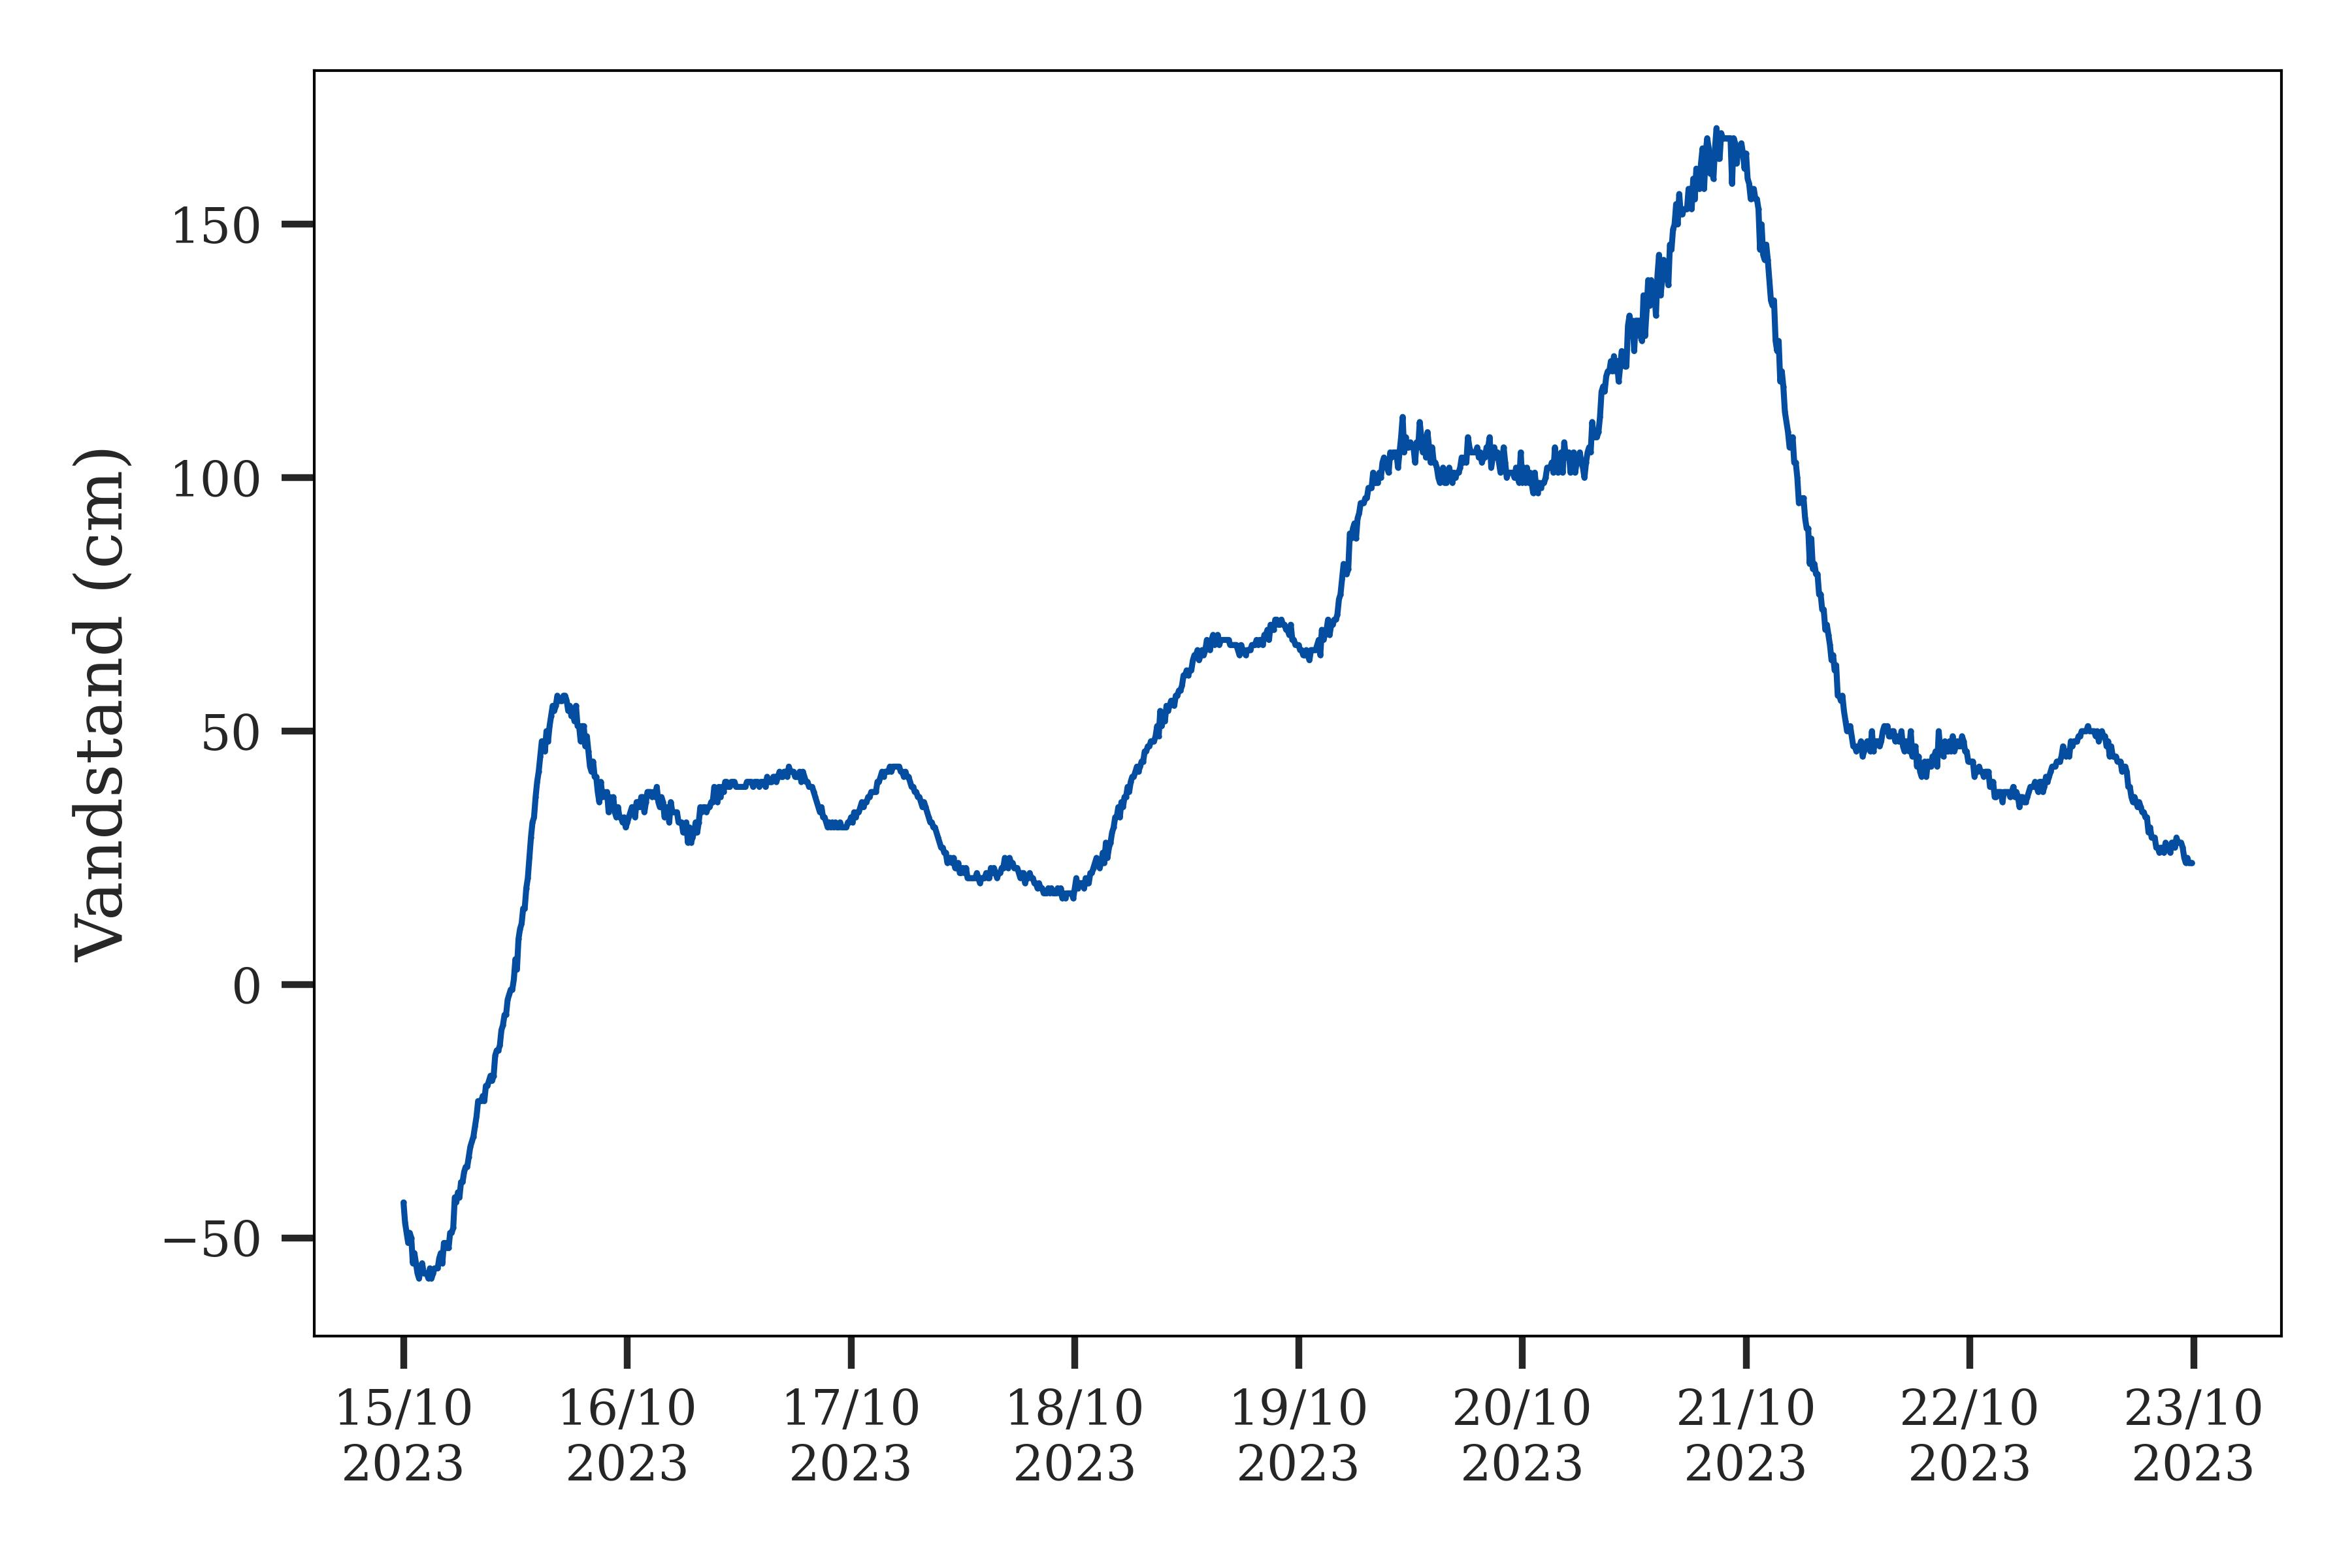
\includegraphics[width=1\textwidth]{images/studieområder/vandstands_grafer/vandstand_praestoe_roedvig_vandstandsplot.jpg}
		\caption{}
		\label{Subfig: Rødvig vandstand}
	\end{subfigure}
	\caption{Officiel målt vandstandsniveau i Aabenraa, Gedser Havn, Hesnæs og Rødvig fra den 15. til 23. oktober. \textbf{(a)} Vandstanden i Aabenraa fra 15. til 23. oktober 2023. \textbf{(b)} Vandstanden i Gedser Havn fra 15. til 23. oktober 2023. \textbf{(c)} Vandstanden i Hesnæs fra 15. til 21. oktober 2023. \textbf{(d)} Vandstanden i Rødvig fra 15. til 23. oktober 2023. Kilde: Data stammer fra DMI og DMIs Frie Data API-ressource.}
	\label{Figur: Vandstandsdata}
\end{figure}

\noindent
\textit{Hesnæs}\\
Hesnæs is a small fishing hamlet on the eastern coast of the island of Falster in the Guldborgsund municipality. Hesnæs mainly serves a fishing and yachting harbour and is the only harbour on the east coast of Falster. Hesnæs is located in between two forests: Corselitze forest to the north and Bønnet forest to the south, both of which extend to sloping cliffs out to the Baltic Sea and form a natural low lying area by the hamlet. \\
Hesnæs was hit particularly hard by the storm surge, where official water levels ruse to 2.10 metres above DVR90. An unofficial measurement reached 2.39 metres above DVR90 at 18:30 UTC October 20th, but the gauge broke shortly after 18:30 UTC (figure \ref{Subfig: Hesnæs vandstand}). Much of Hesnæs harbour was severely damaged by the storm surge due to Hesnæs' exposure towards the Baltic Sea. In particular, the outer pier of the harbour was destroyed by high waves and the mooring bridges were washed ashore. The marina is currently still out of service and the damage to the pier is still visible. \\

\noindent
\textit{Præstø}\\
Præstø is port town in the Vordingborg municipality on the major island of Zealand. The town is located in the southern part of Præstø Fjord, behind the peninsula of Feddet at the bottom of Faxe Bugt. The Tubæk Å, a watercourse that flows from the Tubæk tunnel valley a little south of the town, runs through the central part of the town. Tubæk Å divides Præstø between a northern commercial centre and southern residential area. The town has a population of approximately 4,000 in 2025. \citep{danmarks_statistisk_mobile_nodate} and is the municipality's second largest town.\\
During the storm surge, large parts of Præstøs northern commercial centre were flooded, especially after the sluice gate used to regulate the water levels in Tubæk Å collapsed \citep{uldall_sluseport_2023}. There are no official measurements of the water level in Præstø during the storm, as the nearest measuring station is located further upstream in Tubæk Å. \cite{cowi_praesto_2025} estimates that the water level was approximately 40 centimetres higher than in Rødvig in Stevns municipality around 25 km northeast of Præstø. This gives a water level approximately 2 metres above DVR90 during the storm surge in Præstø. (figure \ref{Subfig: Rødvig vandstand}).

